\documentclass{article}

\usepackage{graphicx}
\usepackage{tikz}
\usepackage{tikzsymbols}
\usetikzlibrary{calc,patterns,shapes.geometric}
\pagestyle{empty}
\usepackage[margin=0pt]{geometry}
\geometry{papersize={14in,12in}}

\def\centerarc[#1](#2)(#3:#4:#5){\draw[#1] ($(#2)+({#5*cos(#3)},{#5*sin(#3)})$) arc (#3:#4:#5);}

\begin{document}
	\begin{figure}
		\centering
		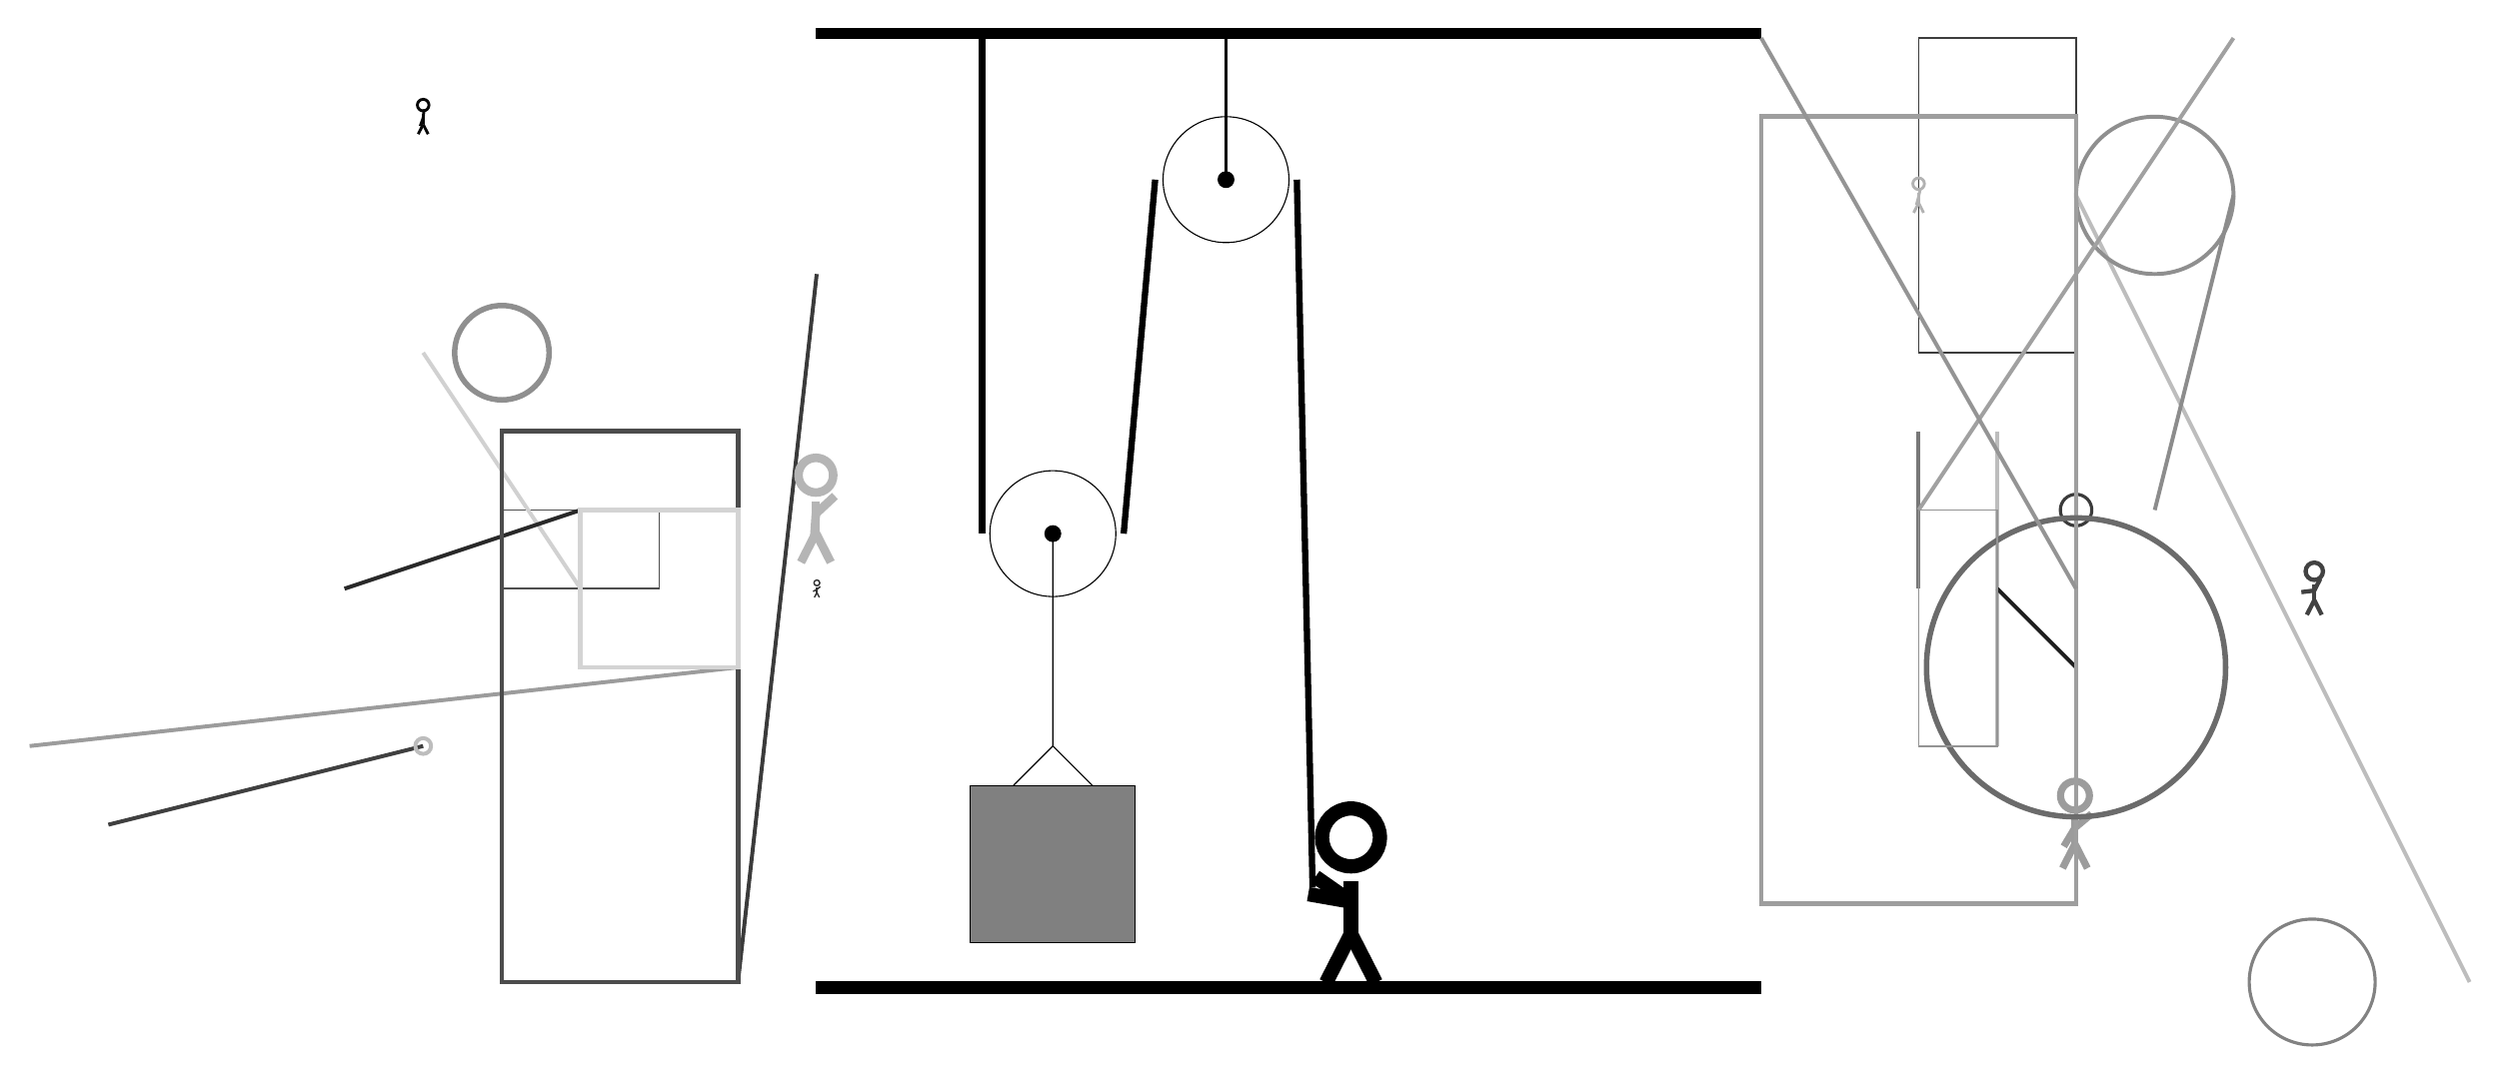
\begin{tikzpicture}
			%%%%% START %%%%%
			
			\draw[fill=black] (-2, 9) rectangle (10, 9.125);
			
			\draw[line width=0.5mm, color=black!75](-7, 0) -- (-11, -1);
			
			\draw[line width=0.5mm, color=black!53](12, 4) -- (12, 2);
			\draw[line width=0.5mm, color=black!26](14, 7) -- (19, -3);
			\draw[line width=0.2mm, color=black!76] (12, 9) rectangle (14, 5);
			\draw[line width=0.2mm, color=black!69] (-4, 2) rectangle (-6, 3);
			\draw[line width=0.5mm, color=black!39](-3, 1) -- (-12, 0);
			\draw [line width=0.5mm, color=black!44](15, 7) circle (1.0);
			\draw[line width=0.5mm, color=black!26](13, 0) -- (13, 4);
			\draw [line width=0.4mm, color=black!77](14, 3) circle (0.2);
			\draw [line width=0.4mm, color=black!49](17, -3) circle (0.8);
			\draw[line width=0.5mm, color=black!37](12, 3) -- (16, 9);
			\node[line width=0.7mm, color=black!39] at (14, -1) {\Strichmaxerl[5][59][40]};
			\draw[line width=0.5mm, color=black!88](13, 2) -- (14, 1);
			
			\node[line width=0.3mm, color=black!74] at (17, 2) {\Strichmaxerl[3][7][63]};
			\draw[line width=0.5mm, color=black!77](-3, -3) -- (-2, 6);
			\draw[line width=0.5mm, color=black!45](15, 3) -- (16, 7);
			
			\node[line width=0.7mm, color=black!97] at (-7, 8) {\Strichmaxerl[2][70][84]};
			\node[line width=0.2mm, color=black!80] at (-2, 2) {\Strichmaxerl[1][30][37]};
			\draw[line width=0.5mm, color=black!18](-7, 5) -- (-5, 2);
			\draw [line width=0.5mm, color=black!26](-7, 0) circle (0.1);
			\draw[line width=0.5mm, color=black!84](-5, 3) -- (-8, 2);
			\draw[line width=0.6mm, color=black!38] (10, -2) rectangle (14, 8);
			\draw [line width=0.7mm, color=black!58](14, 1) circle (1.9);
			\draw[line width=0.6mm, color=black!70] (-3, -3) rectangle (-6, 4);
			\node[line width=0.3mm, color=black!29] at (-2, 3) {\Strichmaxerl[6][86][43]};
			
			\node[line width=0.2mm, color=black!30] at (12, 7) {\Strichmaxerl[2][75][78]};
			\draw[line width=0.2mm, color=black!42] (12, 0) rectangle (13, 3);
			\draw[line width=0.5mm, color=black!42](14, 2) -- (10, 9);
			\draw[line width=0.6mm, color=black!17] (-3, 1) rectangle (-5, 3);
			\draw [line width=0.7mm, color=black!44](-6, 5) circle (0.6);
			
			\draw (3.2, 7.2) circle (0.8);
			\draw[fill=black] (3.2, 7.2) circle (0.1);
			\draw[thick] (3.2, 7.2) -- (3.2, 9);
			
			\draw (1, 2.7) circle (0.8);
			\draw[fill=black] (1, 2.7) circle (0.1);
			
			\draw (1, 2.7) -- (1, 0) -- (0.5, -0.5);
			\draw (1, 0) -- (1.5, -0.5);
			\draw[fill=black!50] (-0.05, -0.5) rectangle (2.05, -2.5);
			
			\draw[line width=0.8mm] (0.1, 9) -- (0.1, 2.7);
			\centerarc[line width=0.8mm](1, 2.7)(180:360:0.9);
			\draw[line width=0.8mm](1.9, 2.7) -- (2.3, 7.2);
			\centerarc[line width=0.8mm](3.2, 7.2)(0:180:0.9);
			\draw[line width=0.8mm](4.1, 7.2) -- (4.3, -1.8);
			
			\node at (4.7, -1.9) {\Strichmaxerl[10][-35][170]};
			
			\draw[fill=black] (-2, -3) rectangle (10, -3.15);
			
			%%%%% END %%%%%
		\end{tikzpicture}
	\end{figure}	
\end{document}